\begin{frame}{Il Modello E/R}
\vspace{.5cm}
\begin{block}{Modello E/R}
Il modello Entit\`a/Associazioni (in inglese \textbf{Entity/Relationships}), \`e uno strumento per analizzare le caratteristiche di una realt\`a in modo indipendente dagli eventi che in essa accadono, ci\`o per costruire un modello concettuale dei dati indipendente dalle applicazioni che li usano.

Si concretizza in una rappresentazione grafica, detta \textbf{schema E/R}.
\end{block}
\pause
Il modello descrive lo schema concettuale di un problema e non si occupa dell'efficienza delle operazioni di manipolazione e ritrovamento dei dati sugli archivi fisici.
\pause

Gli elementi di un modello E/R sono:
\begin{itemize}
    \item entit\`a;
    \item associazioni;
    \item attributi.
\end{itemize}
\end{frame}
%
\begin{frame}{Entit\`a e Associazioni}
\framesubtitle{Entit\`a}
\begin{block}{Entit\`a}
L'\textbf{entit\`a} \`e un oggetto (concreto o astratto) che ha un significato anche quando viene considerato in modo isolato ed \`e di interesse per la realt\`a che si vuole modellare.
\end{block}
\pause
Esempi di entit\`a:
\begin{itemize}
    \item una persona;
    \item un modello di un'automobile;
    \item un movimento contabile;
    \item una prova sostenuta da uno studente;
    \item \ldots
\end{itemize}
\end{frame}
%
\begin{frame}{Entit\`a e Associazioni}
\framesubtitle{Entit\`a}
Le entit\`a possono essere classificate secondo un certo criterio di omogeneit\`a definendo il \textbf{tipo di entit\`a} attraverso un nome.
\pause
\vspace{.3cm}

Esempio:
\begin{itemize}
    \item gli studenti di una scuola sono classificabili nel tipo entit\`a \textit{Studente};
    \item i diversi modelli di automobile sono classificabili nel tipo entit\`a \textit{Automobile}.
\end{itemize}

\pause

\begin{block}{Istanza}
L'\textbf{istanza} di un tipo entit\`a \`e un oggetto concreto che appartiene a quel tipo entit\`a.
\end{block}
\end{frame}
%
\begin{frame}{Entit\`a e Associazioni}
\framesubtitle{Entit\`a}
Nella rappresentazione grafica le entit\`a sono identificate con un rettangolo contenente all'interno il nome dell'entit\`a:

\begin{center}
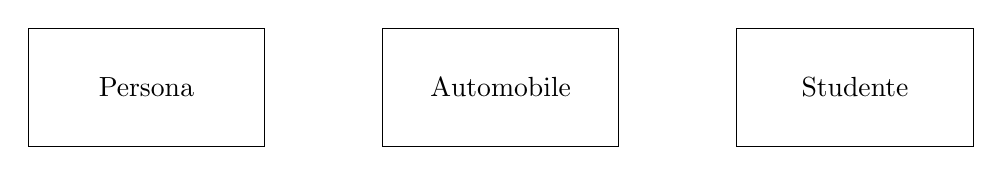
\begin{tikzpicture}
    \uncover<2->{\node[draw, rectangle, minimum width=3cm, minimum height=1.5cm] (persona) at (0, 0) {Persona};}
    \uncover<3->{\node[draw, rectangle, minimum width=3cm, minimum height=1.5cm] (automobile) at (4.5, 0) {Automobile};}
    \uncover<4->{\node[draw, rectangle, minimum width=3cm, minimum height=1.5cm] (studente) at (9, 0) {Studente};}
\end{tikzpicture}
\end{center}
\end{frame}
%
\begin{frame}{Entit\`a e Associazioni}
\framesubtitle{Entit\`a}
In altre parole, le entit\`a sono classi di oggetti che possono esistere autonomamente ai fini del progetto.
\vspace{1cm}

\begin{center}
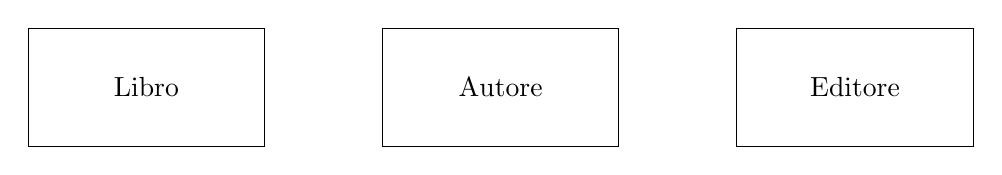
\begin{tikzpicture}
    \uncover<2->{\node[draw, rectangle, minimum width=3cm, minimum height=1.5cm] (libro) at (0, 0) {Libro};}
    \uncover<3->{\node[draw, rectangle, minimum width=3cm, minimum height=1.5cm] (autore) at (4.5, 0) {Autore};}
    \uncover<4->{\node[draw, rectangle, minimum width=3cm, minimum height=1.5cm] (editore) at (9, 0) {Editore};}
\end{tikzpicture}
\end{center}
\end{frame}
%
\begin{frame}{Entit\`a e Associazioni}
\framesubtitle{Associazioni}
\begin{block}{Associazione}
L'\textbf{associazione} (in inglese \textbf{relationship}) \`e un legame che stabilisce un'interazione tra le entit\`a.
\end{block}
\pause
\begin{center}
    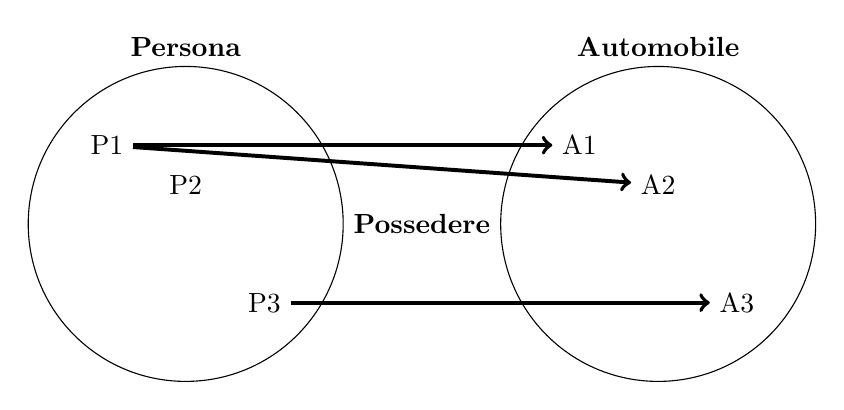
\begin{tikzpicture}
        % Draw the first set as a circle and label it "Persona"
        \node[circle, draw, minimum size=4cm, label=above:{\textbf{Persona}}] (set1) at (0,0) {};
        % Label the points in the first set
        \node at (-1,1) (P1) {P1};
        \node at (0,0.5) (P2) {P2};
        \node at (1,-1) (P3) {P3};
    
        % Draw the second set as a circle and label it "Automobile"
        \node[circle, draw, minimum size=4cm, label=above:{\textbf{Automobile}}] (set2) at (6,0) {};
        % Label the points in the second set
        \node at (5,1) (A1) {A1};
        \node at (6,0.5) (A2) {A2};
        \node at (7,-1) (A3) {A3};
    
        % Draw arrows between points
        \draw[->, line width=.5mm] (P1) -- (A1);
        \draw[->, line width=.5mm] (P1) -- (A2);
        \draw[->, line width=.5mm] (P3) -- (A3);
    
        % Insert the text "Possedere" between the sets
        \node at (3,0) {\textbf{Possedere}};
        
    \end{tikzpicture}
\end{center}
\end{frame}
%
\begin{frame}{Associazioni: alcune osservazioni}
\vspace{-.5cm}
\begin{center}
    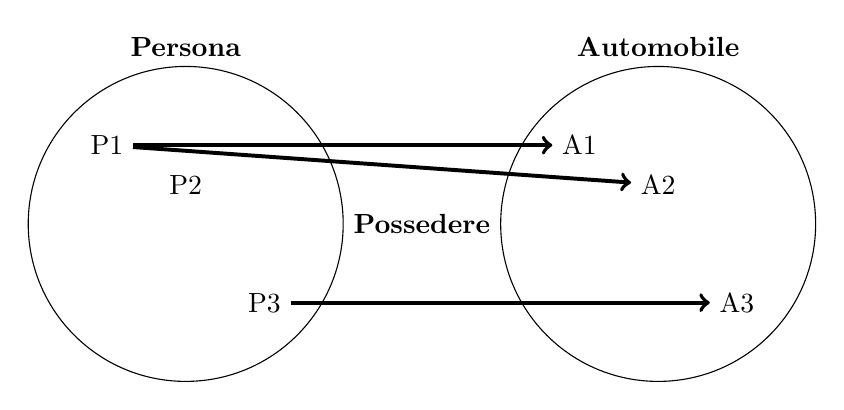
\begin{tikzpicture}
        % Draw the first set as a circle and label it "Persona"
        \node[circle, draw, minimum size=4cm, label=above:{\textbf{Persona}}] (set1) at (0,0) {};
        % Label the points in the first set
        \node at (-1,1) (P1) {P1};
        \node at (0,0.5) (P2) {P2};
        \node at (1,-1) (P3) {P3};
    
        % Draw the second set as a circle and label it "Automobile"
        \node[circle, draw, minimum size=4cm, label=above:{\textbf{Automobile}}] (set2) at (6,0) {};
        % Label the points in the second set
        \node at (5,1) (A1) {A1};
        \node at (6,0.5) (A2) {A2};
        \node at (7,-1) (A3) {A3};
    
        % Draw arrows between points
        \draw[->, line width=.5mm] (P1) -- (A1);
        \draw[->, line width=.5mm] (P1) -- (A2);
        \draw[->, line width=.5mm] (P3) -- (A3);
    
        % Insert the text "Possedere" between the sets
        \node at (3,0) {\textbf{Possedere}};
        
    \end{tikzpicture}
\end{center}
\begin{itemize}[<+->]
    \item 2 entit\`a: Persona con le istanze P1, P2 e P3; Automobile con le istanze A1, A2 e A3;
    \item Un insieme di archi che rappresentano l'associazione di possesso che si viene a stabilire tra le persone e le automobili;
    \item L'associazione ha nome \textit{Possedere} e ha un verso che \`e spacificato tramite le frecce che collegano l'entit\`a \textit{Persona} con l'entit\`a \textit{Automobile}.
\end{itemize}
\end{frame}
%
\begin{frame}{Associazioni: alcune osservazioni}
\vspace{-.8cm}
\begin{center}
    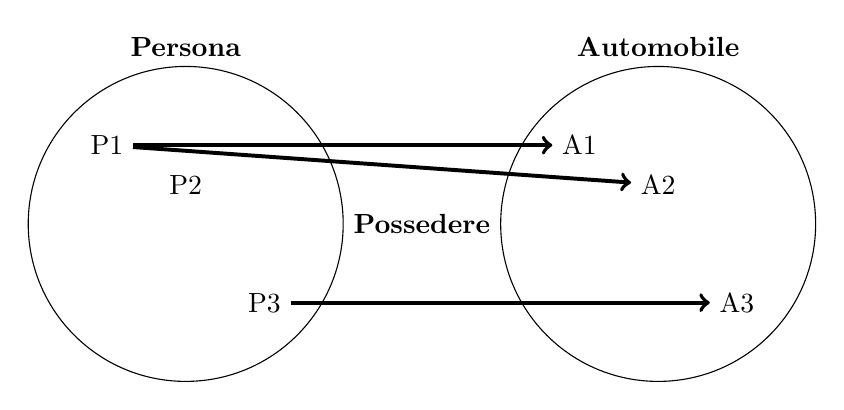
\begin{tikzpicture}
        % Draw the first set as a circle and label it "Persona"
        \node[circle, draw, minimum size=4cm, label=above:{\textbf{Persona}}] (set1) at (0,0) {};
        % Label the points in the first set
        \node at (-1,1) (P1) {P1};
        \node at (0,0.5) (P2) {P2};
        \node at (1,-1) (P3) {P3};
    
        % Draw the second set as a circle and label it "Automobile"
        \node[circle, draw, minimum size=4cm, label=above:{\textbf{Automobile}}] (set2) at (6,0) {};
        % Label the points in the second set
        \node at (5,1) (A1) {A1};
        \node at (6,0.5) (A2) {A2};
        \node at (7,-1) (A3) {A3};
    
        % Draw arrows between points
        \draw[->, line width=.5mm] (P1) -- (A1);
        \draw[->, line width=.5mm] (P1) -- (A2);
        \draw[->, line width=.5mm] (P3) -- (A3);
    
        % Insert the text "Possedere" between the sets
        \node at (3,0) {\textbf{Possedere}};
        
    \end{tikzpicture}
\end{center}
\begin{itemize}[<+->]
    \item P1 possiede le automobili A1 e A2;
    \item P2 non possiede auto;
    \item P3 possiede l'auto A3;
    \item Tra \textit{Persona} e \textit{Automobile} sussiste l'associazione \textit{Possedere}.
    \item Una persona pu\`o possedere una o pi\`u automobili, ma un'automobile \`e posseduta da una sola persona.
\end{itemize}
\end{frame}
%
\begin{frame}{Associazioni}
In altre parole, le associazioni sono i diversi tipi di relazioni che intercorrono tra le entit\`a.
\vspace{1cm}
\begin{center}
\begin{tikzpicture}
    % First flattened rhombus with "utilizzo", initially hidden
    \uncover<2->{
        \node[draw, diamond, minimum width=4cm, minimum height=2cm, text width=2cm, align=center] at (0,0) {Utilizzo};
    }
    
    % Second flattened rhombus with "parentela", initially hidden
    \uncover<3->{
        \node[draw, diamond, minimum width=4cm, minimum height=2cm, text width=2cm, align=center] at (5,0) {Parentela};
    }
\end{tikzpicture}
\end{center}
\end{frame}
%
\begin{frame}{Associazioni: convenzioni}

\begin{itemize}
    \item La rappresentazione grafica convenzionalmente usata per indicare un'associazione \`e una linea che unisce le entit\`a interessate;
    \item Il nome compare sulla linea con il simbolo della punta di una freccia per indicare il senso di lettura dell'associazione;
\end{itemize}
\pause
\begin{center}
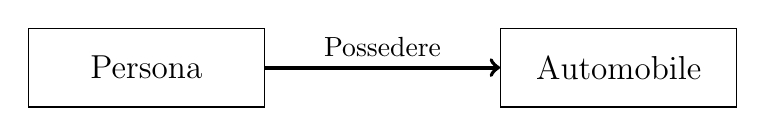
\begin{tikzpicture}
    % Define styles for shapes
    \tikzstyle{rectangle} = [draw, minimum width=3cm, minimum height=1cm, text centered, font=\large]

    % Draw the two rectangles
    \node[rectangle] (persona) at (0,0) {Persona};
    \node[rectangle] (automobile) at (6,0) {Automobile};

    % Draw the arrow between the rectangles with the label "Possedere"
    \draw[->, line width=0.5mm] (persona) -- node[above] {Possedere} (automobile);
    
\end{tikzpicture}
\end{center}
\pause
\begin{block}{Nota bene}
    Di norma i nomi delle entit\`a sono \textbf{sostantivi} mentre i nomi delle associazioni sono \textbf{verbi} (vanno bene anche sostantivi).
    \pause

    \`E inoltre necessario considerare nome e verso di lettura dell'associazione!
\end{block}
\end{frame}
%
\begin{frame}{Associazioni: convenzioni - osservazioni}
\begin{center}
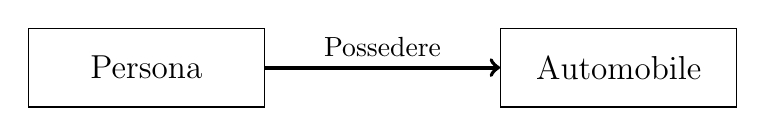
\begin{tikzpicture}
    % Define styles for shapes
    \tikzstyle{rectangle} = [draw, minimum width=3cm, minimum height=1cm, text centered, font=\large]

    % Draw the two rectangles
    \node[rectangle] (persona) at (0,0) {Persona};
    \node[rectangle] (automobile) at (6,0) {Automobile};

    % Draw the arrow between the rectangles with the label "Possedere"
    \draw[->, line width=0.5mm] (persona) -- node[above] {Possedere} (automobile);
    
\end{tikzpicture}
\end{center}
\begin{itemize}[<+->]
    \item Tra l'entit\`a \textit{Persona} e l'entit\`a \textit{Automobile} esiste l'associazione \textit{Possedere};
    \item L'associazione tra le entit\`a \textit{Automobile} e l'entit\`a \textit{Persona} pu\`o essere descritta mediante la forma passiva del verbo che rappresenta la precedente associazione;
    \item Quindi tra l'entit\`a \textit{Automobile} e l'entit\`a \textit{Persona} esiste l'associazione \textit{EsserePosseduta} che non \`e rappresentata esplicitamente nel grafico.
    \item Il nome dell'associazione rappresenta \textbf{solo uno} dei due versi dell'associazione, quello nel quale la lettura ha senso;
    \item Il verso \`e precisato con il simbolo a forma di punta di freccia posto accanto al nome.
\end{itemize}
\end{frame}
%
\begin{frame}{Associazioni: convenzioni}
Esistono diverse rappresentazioni formali del modello ER.

Noi useremo il simbolismo della linea non orientata ma con un rombo a met\`a di questa linea:
\begin{center}
\begin{tikzpicture}[remember picture]
    % Define styles for shapes
    \tikzstyle{rectangle} = [draw, minimum width=3cm, minimum height=1cm]
    \tikzstyle{rhombus} = [draw, diamond, minimum width=3cm, minimum height=1cm, aspect=2]
    % Draw shapes
    \node[rectangle] (rect1) at (2, -0.5) {Persona};
    \node[rhombus] (rhombus) at (7, -0.5) {Possiede};
    \node[rectangle] (rect2) at (12, -0.5) {Automobile};
    % Draw arrows
    \draw (rect1) -- (rhombus) node[midway, above] {};
    \draw (rhombus) -- (rect2) node[midway, above] {};
\end{tikzpicture}
\end{center}
\end{frame}
%
\begin{frame}{Associazioni: Grado}
Le associazioni hanno un \textbf{grado}.

\begin{itemize}
    \onslide<1-> \item Il grado \`e dato dal numero di entit\`a che partecipano all'associazione;
    \onslide<2-> \item L'associazione tra \textit{Automobile} e \textit{Persona} ha grado 2 e viene detta \textbf{associazione binaria};
\end{itemize}
\onslide<2->{
\begin{center}
    \begin{tikzpicture}[remember picture]
        % Define styles for shapes
        \tikzstyle{rectangle} = [draw, minimum width=3cm, minimum height=1cm]
        \tikzstyle{rhombus} = [draw, diamond, minimum width=3cm, minimum height=1cm, aspect=2]
        % Draw shapes
        \node[rectangle] (rect1) at (2, -0.5) {Persona};
        \node[rhombus] (rhombus) at (7, -0.5) {Possiede};
        \node[rectangle] (rect2) at (12, -0.5) {Automobile};
        % Draw arrows
        \draw (rect1) -- (rhombus) node[midway, above] {};
        \draw (rhombus) -- (rect2) node[midway, above] {};
    \end{tikzpicture}
    \end{center}
}
\begin{itemize}
\onslide<3-> \item Naturalmente esistono associazioni di grado 1, 3 e di grado superiore.
\end{itemize}
\end{frame}
%
\begin{frame}{Associazioni: pi\`u di una}
Due entit\`a possono essere collegate da pi\`u di un'associazione:
\begin{center}
    \begin{tikzpicture}
        % Define styles for shapes
        \tikzstyle{rectangle} = [draw, minimum width=3cm, minimum height=1cm, text centered, font=\large]
    
        % Draw the two rectangles
        \node[rectangle] (docente) at (0,0) {Docente};
        \node[rectangle] (classe) at (6,0) {Classe};
    
        % Draw the labels above and below "Docente"
        \node[above=0.1cm of docente] {\small insegnante};
        \node[below=0.1cm of docente] {\small coordinatore};
    
        % Draw the arrows between the rectangles with the labels "Insegnare" and "Coordinare"
        \draw[->, line width=0.5mm] (docente) -- node[above] {Insegnare} (classe);
        \draw[->, line width=0.5mm] (docente) -- ++(6, -1.5) node[midway, below=0.25cm] {Coordinare} -- (classe);
    
    \end{tikzpicture}
\end{center}
\pause
\textit{insegnante} e \textit{coordinatore} sono i nomi dei due ruoli che il \textit{docente} pu\`o assumere nelle 2 associazioni.
\end{frame}
%
\begin{frame}{Associazioni: Le associazione ricorsive}
Ci sono associazioni tra un'entit\`a e se stessa:

\pause
{
Consideriamo l'entit\`a \textit{Persona} e l'associazione di maternit\`a (o paternit\`a) che collega una madre con i propri figli (o un padre con i propri figli):
\begin{center}
    \begin{tikzpicture}
        % Define styles for shapes
        \tikzset{
            rectangle/.style={draw, minimum width=3cm, minimum height=1cm},
            rhombus/.style={draw, diamond, minimum width=3cm, minimum height=1cm, aspect=2}
        }
        % Draw shapes
        \node[rectangle] (rect1) at (2, -0.5) {Persona};
        \node[rhombus] (rhombus) at (7, -0.5) {Essere madre di};
        % Draw arrows
        \draw[-] (rect1) -- (rhombus) node[midway, above] {};
        \draw[-] (rhombus) -- (rect1) node[midway, below] {};
        % Additional arrows
        \draw[-] (rhombus) -- ++(0,-1) -| (rect1) node[pos=0.25, below] {};
        % Add text "Madre" above Persona and "Figlio" below Persona
        \node[above right=-0.1cm of rect1] {\small Madre};
        \node[below right=-0.1cm of rect1] {\small Figlio};
    \end{tikzpicture}
\end{center}
}
\pause
\begin{block}{Associazioni ricorsive}
In queste associazioni l'entit\`a \textit{Persona} partecipa con ruoli diversi all'associazione.

Le associazioni di questo tipo si dicono \textbf{associazioni ricorsive}.
\end{block}

\end{frame}
%
\begin{frame}{Associazioni: Le associazione ricorsive}
Altro esempio di associazione ricorsiva nella quale l'entit\`a \textit{Dipendente} partecipa all'associazione \textit{Coordinare} nel duplice ruolo di \textit{Supervisore} e di \textit{Collaboratore}.
\begin{center}
    \begin{tikzpicture}
        % Define styles for shapes
        \tikzset{
            rectangle/.style={draw, minimum width=3cm, minimum height=1cm},
            rhombus/.style={draw, diamond, minimum width=3cm, minimum height=1cm, aspect=2}
        }
        % Draw shapes
        \node[rectangle] (rect1) at (2, -0.5) {Dipendente};
        \node[rhombus] (rhombus) at (7, -0.5) {Coordinare};
        % Draw arrows
        \draw[-] (rect1) -- (rhombus) node[midway, above] {};
        \draw[-] (rhombus) -- (rect1) node[midway, below] {};
        % Additional arrows
        \draw[-] (rhombus) -- ++(0,-1) -| (rect1) node[pos=0.25, below] {};
        
        \node[above right=-0.1cm of rect1] {\small Supervisore};
        \node[below right=-0.1cm of rect1] {\small Collaboratore};
    \end{tikzpicture}
\end{center}

\end{frame}
%
\begin{frame}{Attributi}
\begin{minipage}{0.9\textwidth}
\begin{block}{Gli attributi}
Le propriet\`a delle entit\`a e delle associazioni sono descritte attraverso gli \textbf{attributi}.
\end{block}
\end{minipage}
\pause
\newline
\\Caratteristiche principali degli attributi:
\begin{itemize}[<+->]
    \item Il \textbf{formato} di un attributo indica il tipo di valori che assume;
    
    3 formati di base: carattere, numerico, data/ora;
    \item La \textbf{dimensione} indica la quantit\`a massima di caratteri o cifre inseribili quando si valorizza l'attributo;
    \item \textbf{Opzionalit\`a}: l'attributo \`e obbligatorio se deve avere valore non nullo (es. codice fiscale in un' anagrafe), facoltativo se sono accettabili valori nulli (esempio, titolo di studio).
\end{itemize}
\end{frame}
%
\begin{frame}{Attributi}
\begin{itemize}[<+->]
    \item Il valore \textbf{nullo} rappresenta un'informazione mancante in quanto inapplicabile o sconosciuta;
    \item I diversi valori assunti dagli attributi determinano le diverse \textbf{istanze} dell'entit\`a;
    \item L'insieme dei possibili valori assunti da un attributo si chiama  \textbf{dominio} dell'attributo;
    \item I valori appartenenti al dominio sono omogenei tra loro, cio\`e sono dello stesso tipo.
\end{itemize}
\end{frame}
%
\begin{frame}{Attributi: un esempio}
\begin{minipage}[t]{0.7\linewidth}
    Quali potrebbero essere gli attributi dell'entit\`a \textit{Automobile}?
    \pause
    \begin{itemize}[<+->]
        \item Modello;
        \item Produttore;
        \item Cilindrata;
        \item Potenza;
        \item PrezzoListino;
        \item \ldots
    \end{itemize}
\end{minipage}%
\begin{minipage}[t]{0.2\linewidth}
    \pause
    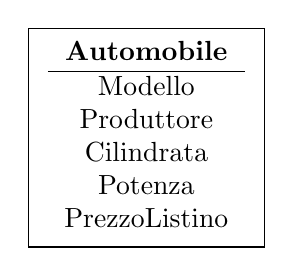
\begin{tikzpicture}[remember picture]
        % Define styles for shapes
        \tikzstyle{rectangle} = [draw, minimum width=3cm, minimum height=1cm]
        
        % Draw shapes
        \node[rectangle] (rect1) at (1.5, -1) {
                \begin{tabular}{c}
                    \textbf{Automobile} \\
                    \hline
                    Modello \\
                    Produttore \\
                    Cilindrata \\
                    Potenza \\
                    PrezzoListino \\
                \end{tabular}
        };
    \end{tikzpicture}
\end{minipage}
\end{frame}
%
\begin{frame}{Attributi sulle associazioni}
Anche le associazioni possono avere attributi:
\begin{center}
    \begin{tikzpicture}[remember picture]
        % Define styles for shapes
        \tikzstyle{rectangle} = [draw, minimum width=3cm, minimum height=1cm]
        \tikzstyle{rhombus} = [draw, diamond, minimum width=3cm, minimum height=1cm, aspect=2]
        % Draw shapes
        \node[rectangle] (rect1) at (1.5, -1) {
                \begin{tabular}{c}
                    \textbf{Persona} \\
                    \hline
                    CodiceFiscale \\
                    Cognome \\
                    Nome \\
                    DataNascita \\
                    Indirizzo \\
                \end{tabular}
        };
        \node[rhombus] (rhombus) at (7, -1) {Acquistare};
        \node[rectangle] (rect2) at (11.5, -1) {
                \begin{tabular}{c}
                    \textbf{Automobile} \\
                    \hline
                    Modello \\
                    Produttore \\
                    Cilindrata \\
                    Potenza \\
                    PrezzoListino \\
                \end{tabular}
            };
         % Fornire rectangle under the rhombus
         \node[rectangle] (rect3) at (7, -3) {
            \begin{tabular}{c}
                 \\
                \hline
                DataAcquisto \\
                PrezzoAcquisto \\
            \end{tabular}
        };
        % Draw arrows
        \draw (rect1) -- (rhombus) node[midway, above] {};
        \draw (rhombus) -- (rect2) node[midway, above] {};
         % line from rhombus to the Acquistare rectangle
         \draw (rhombus) -- (rect3) node[midway, right] {};
    \end{tikzpicture}
    \end{center}
\end{frame}
%
\begin{frame}{Attributi sulle associazioni}
\`E importante osservare che la presenza di un'associazione con attributi potrebbe essere indicativa della presenza di un'altra entit\`a oltre a quelle identificate:
\pause
\begin{center}
    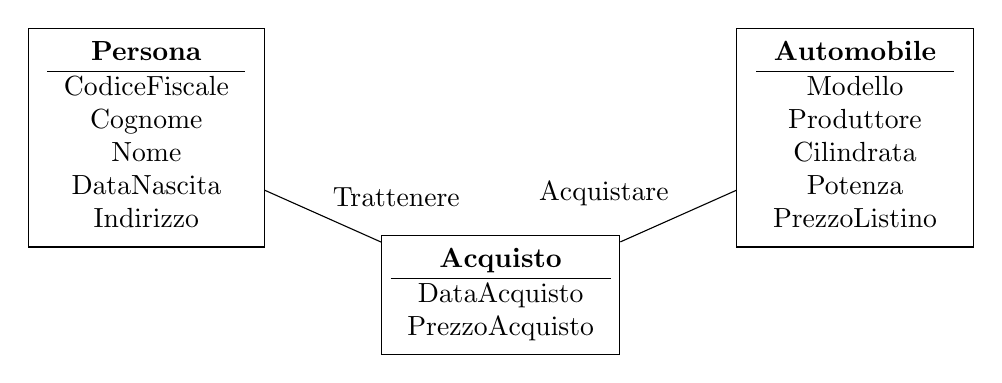
\begin{tikzpicture}[remember picture]
        % Define styles for shapes
        \tikzset{
            rectangle/.style={draw, minimum width=3cm, minimum height=1cm},
            rhombus/.style={draw, diamond, minimum width=3cm, minimum height=1cm, aspect=2}
        }
        % Draw shapes with increased distance
        \node[rectangle] (rect1) at (0, -1) {
                \begin{tabular}{c}
                    \textbf{Persona} \\
                    \hline
                    CodiceFiscale \\
                    Cognome \\
                    Nome \\
                    DataNascita \\
                    Indirizzo \\
                \end{tabular}
        };
        \node[rectangle] (rect2) at (9, -1) {
                \begin{tabular}{c}
                    \textbf{Automobile} \\
                    \hline
                    Modello \\
                    Produttore \\
                    Cilindrata \\
                    Potenza \\
                    PrezzoListino \\
                \end{tabular}
            };
         % Fornire rectangle under the rhombus
         \node[rectangle] (rect3) at (4.5, -3) {
            \begin{tabular}{c}
                \textbf{Acquisto} \\
                \hline
                DataAcquisto \\
                PrezzoAcquisto \\
            \end{tabular}
        };
        % Draw arrows
        \draw (rect1) -- (rect3) node[midway, above right] {Trattenere};
        \draw (rect3) -- (rect2) node[midway, above left] {Acquistare};
    \end{tikzpicture}
\end{center}
\end{frame}
%
\begin{frame}{Attributi}
Una regola molto importante  richiede di definire solo gli attributi elementari e quindi di non definire gli attributi che si ottengono con le elaborazioni, cio\`e gli \textbf{attributi derivati}.
\pause
\newline
\\Perch\`e dovremo evitare di definire attributi derivati?
\pause
\newline
\\Perch\`e il mancato rispetto della regola provoca inefficienza dovuta alle elaborazioni necessarie per aggiornare questo tipo di attributi!
\pause

Alcuni esempi:
\begin{itemize}
    \item l' et\`a di una persona \`e un attributo derivato dall'attributo elementare della data di nascita;
    \item il saldo di un conto corrente \`e derivato dalla somma algebrica degli importi dei movimenti effettuati sul conto.
    \item \ldots
\end{itemize}
\end{frame}
%
\begin{frame}{Attributi: Chiave primaria}
\vspace{-.9cm}

\begin{minipage}{0.9\textwidth}
\begin{block}{Chiave primaria}
Si indica con il termine \textbf{chiave} o \textbf{chiave primaria} (primary key) un insieme minimale di attributi che permettono di distinguere tra loro le istanze di una stessa entit\`a.
\end{block}
\end{minipage}
\pause
\newline
\\Alcuni esempi:
\begin{itemize}[<+->]
    \item il codice di un prodotto;
    \item la matricola di un dipendente;
    \item la chiave composta del codice studente insieme alla data e al codice della materia per le prove scolastiche;
    \item \ldots
\end{itemize}
\pause

Nel caso delle 2 entit\`a \textit{Persona} e \textit{Automobile} gli attributi CodiceFiscale e Modello sono rispettivamente le chiavi primarie per le entit\`a.
\end{frame}
%
\begin{frame}{Attributi}
In altre parole, gli attributi sono le propriet\`a di cui vogliamo tenere conto per ogni entit\`a.
\vspace{1.8cm}

\begin{center}
\begin{tikzpicture}[remember picture, overlay]
    % Define styles for shapes
    \tikzstyle{rectangle} = [draw, minimum width=3cm, minimum height=1cm]
    % Draw shapes
    \node[rectangle] (rect1) at (0, 0) {Persona};
    % Draw attribute line with bullet for "nome"
    \uncover<2->{\draw[decoration={markings,mark=at position 1 with {\draw[white, fill=white] circle [radius=2pt];}},postaction={decorate}] (rect1.west) -- +(-1,0) node[midway, left] {\hspace{-2.1cm}nome};
    \draw[white, fill=white] (rect1.west) ++(-1,0) circle [radius=2pt];
    \draw (rect1.west) ++(-1,0) circle [radius=2pt];}
    % Define a new starting point for the line for "cognome"
    \uncover<3->{\coordinate (startCognome) at ($(rect1.west) + (0,0.2)$);
    % Define a new point for drawing the line for "cognome"
    \coordinate (aboveLine) at ($(rect1.west) + (-1,0.7)$); % Adjust the vertical distance here
    % Draw attribute line with bullet for "cognome"
    \draw[decoration={markings,mark=at position 1 with {\draw[white, fill=white] circle [radius=2pt];}},postaction={decorate}] (startCognome) -- (aboveLine);
    \draw[white, fill=white] (aboveLine) circle [radius=2pt];
    \draw (aboveLine) circle [radius=2pt];
    \node[left] at (aboveLine) {cognome};}
    \uncover<4->{\coordinate (data) at ($(rect1.west) + (0.1,0.5)$);
    \coordinate (aboveLine) at ($(rect1.west) + (-0.7,1.5)$);
    \draw[decoration={markings,mark=at position 1 with {\draw[white, fill=white] circle [radius=2pt];}},postaction={decorate}] (data) -- (aboveLine);
    \draw[white, fill=white] (aboveLine) circle [radius=2pt];
    \draw (aboveLine) circle [radius=2pt];
    \node[above] at (aboveLine) {dataNascita};}
    \uncover<5->{\coordinate (tel) at ($(rect1.west) + (1,0.5)$);
    \coordinate (aboveLine) at ($(rect1.west) + (1,1.5)$);
    \draw[decoration={markings,mark=at position 1 with {\draw[white, fill=white] circle [radius=2pt];}},postaction={decorate}] (tel) -- (aboveLine) node[right,font=\tiny] {(1,N)};
    \draw[white, fill=white] (aboveLine) circle [radius=2pt];
    \draw (aboveLine) circle [radius=2pt];
    \node[above] at (aboveLine) {tel};}
    \uncover<6->{\coordinate (indirizzo) at ($(rect1.west) + (2,0.5)$);
    \coordinate (aboveLine) at ($(rect1.west) + (2.5,1.5)$);
    \draw[decoration={markings,mark=at position 1 with {\draw[white, fill=white] circle [radius=2pt];}},postaction={decorate}] (indirizzo) -- (aboveLine);
    \draw[white, fill=white] (aboveLine) circle [radius=2pt];
    \draw (aboveLine) circle [radius=2pt];
    \node[above] at (aboveLine) {indirizzo};}
\end{tikzpicture}  
\end{center}
\end{frame}
%
\begin{frame}{Attributi}
In altre parole, gli attributi sono le propriet\`a di cui vogliamo tenere conto per ogni entit\`a.
\vspace{1.8cm}

\begin{center}
\begin{tikzpicture}[remember picture, overlay]
    % Define styles for shapes
    \tikzstyle{rectangle} = [draw, minimum width=3cm, minimum height=1cm]
    
    % Draw shapes
    \node[rectangle] (rect1) at (0, 0) {Persona};
    
    % Draw attribute line with bullet for "nome"
    \draw[decoration={markings,mark=at position 1 with {\draw[white, fill=white] circle [radius=2pt];}},postaction={decorate}] (rect1.west) -- +(-1,0) node[midway, left] {\hspace{-2.1cm}nome};
    \draw[white, fill=white] (rect1.west) ++(-1,0) circle [radius=2pt];
    \draw (rect1.west) ++(-1,0) circle [radius=2pt];
    
    % Define a new starting point for the line for "cognome"
    \coordinate (startCognome) at ($(rect1.west) + (0,0.2)$);
    % Define a new point for drawing the line for "cognome"
    \coordinate (aboveLine) at ($(rect1.west) + (-1,0.7)$); % Adjust the vertical distance here
    % Draw attribute line with bullet for "cognome"
    \draw[decoration={markings,mark=at position 1 with {\draw[white, fill=white] circle [radius=2pt];}},postaction={decorate}] (startCognome) -- (aboveLine);
    \draw[white, fill=white] (aboveLine) circle [radius=2pt];
    \draw (aboveLine) circle [radius=2pt];
    \node[left] at (aboveLine) {cognome};
    
    % Coordinate and draw line for "dataNascita"
    \coordinate (data) at ($(rect1.west) + (0.1,0.5)$);
    \coordinate (aboveLineData) at ($(rect1.west) + (-0.7,1.5)$);
    \draw[decoration={markings,mark=at position 1 with {\draw[white, fill=white] circle [radius=2pt];}},postaction={decorate}] (data) -- (aboveLineData);
    \draw[white, fill=white] (aboveLineData) circle [radius=2pt];
    \draw (aboveLineData) circle [radius=2pt];
    \node[above] at (aboveLineData) {dataNascita};
    
    % Coordinate and draw line for "tel"
    \coordinate (tel) at ($(rect1.west) + (1,0.5)$);
    \coordinate (aboveLineTel) at ($(rect1.west) + (1,1.5)$);
    \draw[decoration={markings,mark=at position 1 with {\draw[white, fill=white] circle [radius=2pt];}},postaction={decorate}] (tel) -- (aboveLineTel) node[right,font=\tiny] {(1,N)};
    \draw[white, fill=white] (aboveLineTel) circle [radius=2pt];
    \draw (aboveLineTel) circle [radius=2pt];
    \node[above] at (aboveLineTel) {tel};
    
    % Calculate the center of the circle
    \coordinate (centerIndirizzo) at ($(rect1.east) + (1.5,0.5)$); % Adjust position as needed
    
    \draw (centerIndirizzo) circle [x radius=1cm, y radius=0.3cm];
    
    % Calculate the endpoint of the line to connect to the rectangle
    \coordinate (lineEnd) at ($(centerIndirizzo) - (1cm, 0)$);
    
    % Draw the line connecting the circle and the rectangle
    \draw[decoration={markings,mark=at position 1 with},postaction={decorate}] (rect1.east) -- (lineEnd);
    
    % Add the label inside the circle
    \node[font=\small, inner sep=0](ind) at (centerIndirizzo) {indirizzo};
    
    \uncover<2->{\coordinate (indC) at ($(ind.north west) + (0,0.1)$);
    \coordinate (aboveLine) at ($(ind.west) + (-0.7,1)$);
    \draw[decoration={markings,mark=at position 1 with {\draw[white, fill=white] circle [radius=2pt];}},postaction={decorate}] (indC) -- (aboveLine);
    \draw[white, fill=white] (aboveLine) circle [radius=2pt];
    \draw (aboveLine) circle [radius=2pt];
    \node[above] at (aboveLine) {via};}

    \uncover<3->{\coordinate (numCiv) at ($(ind.north) + (0,0.15)$);
    \coordinate (aboveLine) at ($(ind.north) + (0,1)$);
    \draw[decoration={markings,mark=at position 1 with {\draw[white, fill=white] circle [radius=2pt];}},postaction={decorate}] (numCiv) -- (aboveLine);
    \draw[white, fill=white] (aboveLine) circle [radius=2pt];
    \draw (aboveLine) circle [radius=2pt];
    \node[above] at (aboveLine) {numCiv};}
    \uncover<4->{\coordinate (CAP) at ($(ind.north east) + (0,0.1)$);
    \coordinate (aboveLine) at ($(ind.north east) + (1,0.8)$);
    \draw[decoration={markings,mark=at position 1 with {\draw[white, fill=white] circle [radius=2pt];}},postaction={decorate}] (CAP) -- (aboveLine);
    \draw[white, fill=white] (aboveLine) circle [radius=2pt];
    \draw (aboveLine) circle [radius=2pt];
    \node[above] at (aboveLine) {CAP};}

    \uncover<4->{\coordinate (cf) at ($(rect1.west) + (0,-0.3)$);
    \coordinate (aboveLine) at ($(rect1.west) + (-0.7,-1)$);
    \draw[decoration={markings,mark=at position 1 with {\draw[black] circle [radius=2pt];}},postaction={decorate}] (cf) -- (aboveLine);
    \draw[black, fill=black] (aboveLine) circle [radius=2pt];
    \draw (aboveLine) circle [radius=2pt];
    \node[left] at (aboveLine) {CF};}
\end{tikzpicture}
\end{center}
\end{frame}
%
\begin{frame}{Attributi}
Un altro esempio:
\vspace{1.8cm}

\begin{center}
\begin{tikzpicture}[remember picture, overlay]
    % Define styles for shapes
    \tikzstyle{rectangle} = [draw, minimum width=3cm, minimum height=1cm]
    
    % Draw shapes
    \node[rectangle] (rect1) at (0, 0) {Automobile};
    
    % Draw attribute line with bullet for "Modello"
    \draw[decoration={markings,mark=at position 1 with {\draw[black, fill=white] circle [radius=2pt];}},postaction={decorate}] (rect1.west) -- +(-1,0) node[midway, left] {\hspace{-2.5cm}Modello};
    \draw[white, fill=black] (rect1.west) ++(-1,0) circle [radius=2pt];
    \draw (rect1.west) ++(-1,0) circle [radius=2pt];
    
    % Define a new starting point for the line for "Produttore"
    \coordinate (startProduttore) at ($(rect1.west) + (0,0.2)$);
    % Define a new point for drawing the line for "Produttore"
    \coordinate (aboveLine) at ($(rect1.west) + (-1,0.7)$); % Adjust the vertical distance here
    % Draw attribute line with bullet for "Produttore"
    \draw[decoration={markings,mark=at position 1 with {\draw[white, fill=white] circle [radius=2pt];}},postaction={decorate}] (startProduttore) -- (aboveLine);
    \draw[white, fill=white] (aboveLine) circle [radius=2pt];
    \draw (aboveLine) circle [radius=2pt];
    \node[left] at (aboveLine) {Produttore};
    
    % Coordinate and draw line for "Cilindrata"
    \coordinate (data) at ($(rect1.west) + (0.1,0.5)$);
    \coordinate (aboveLineCilindrata) at ($(rect1.west) + (-0.7,1.5)$);
    \draw[decoration={markings,mark=at position 1 with {\draw[white, fill=white] circle [radius=2pt];}},postaction={decorate}] (data) -- (aboveLineCilindrata);
    \draw[white, fill=white] (aboveLineCilindrata) circle [radius=2pt];
    \draw (aboveLineCilindrata) circle [radius=2pt];
    \node[above] at (aboveLineCilindrata) {Cilindrata};
    
    % Coordinate and draw line for "PrezzoListino"
    \coordinate (prezzoListino) at ($(rect1.west) + (1,0.5)$);
    \coordinate (aboveLinePrezzoListino) at ($(rect1.west) + (1,2.5)$);
    \draw[decoration={markings,mark=at position 1 with {\draw[white, fill=white] circle [radius=2pt];}},postaction={decorate}] (tel) -- (aboveLinePrezzoListino) node[right,font=\tiny] {};
    \draw[white, fill=white] (aboveLinePrezzoListino) circle [radius=2pt];
    \draw (aboveLinePrezzoListino) circle [radius=2pt];
    \node[above] at (aboveLinePrezzoListino) {prezzoListino};
\end{tikzpicture}  
\end{center}
\end{frame}
%
\begin{frame}{Le associazioni tra entit\`a}
\begin{block}{Molteplicit\`a di un'associazione}
La \textbf{molteplicit\`a di un'associazione} \`e il numero di possibili istanze di un'entit\`a che viene messo in corrispondenza con un'istanza dell'altra entit\`a che partecipa all'associazione.
\end{block}
\pause
Il numero minimo e massimo di possibili istanze viene rappresentato mediante una coppia di valori separati da punti: 
\begin{itemize}
    \item 1..1
    \item 0..1
    \item 1..N
\end{itemize}
\end{frame}
%
\begin{frame}{Le associazioni tra entit\`a}
Al valore minimo e massimo sono associati gli importanti concetti di \textbf{obbligatoriet\`a} e \textbf{cardinalit\`a} dell'associazione:
\begin{itemize}[<+->]
    \item Il valore minimo assume, in genere, uno dei due valori 0 e 1.
    \begin{itemize}
        \item Lo 0 indica che la partecipazione \`e \textbf{facoltativa};
        \item 1 indica che la partecipazione \`e \textbf{obbligatoria}.
    \end{itemize}
    \item Il valore massimo definisce la \textbf{cardinalit\`a} della partecipazione all'assocazione.
    
    Esso assume, in genere uno dei valori 1 oppure N per indicare una o molte partecipazioni all'associazione.
\end{itemize}
\end{frame}
%
\begin{frame}{Le associazioni tra entit\`a}
\vspace{.5cm}
La cardinalit\`a pu\`o quindi essere \textbf{a uno} oppure \textbf{a molti} e pertanto le associazioni tra due entit\`a si classificano nei seguenti tipi:
\begin{itemize}[<+->]
    \item associazione \textbf{uno a uno} o biunivoca, indicata con \textbf{1:1}
    \item associazione \textbf{uno a molti} o semplice, indicata con \textbf{1:N}
    \item associazione \textbf{molti a molti} o complessa, indicata con \textbf{N:N}
\end{itemize}
\begin{block}{Nota bene}
Non \`e sempre facile attribuire questi valori e solo un attento esame della specifica situazione permette di definirli con esattezza.
\pause
\newline
\\Metodo utile per risolvere i dubbi: rappresentare l'associazione con insiemi di istanze delle entit\`a collegate con archi.
\end{block}
\end{frame}
%
\begin{frame}{Associazione 1 : 1 o biunivoca}
\begin{minipage}{0.9\textwidth}
\begin{block}{Associazione uno a uno}
Un'associazione si dice \textbf{uno a uno}, o biunivoca, e si indica con \textbf{1:1}, quando ogni istanza della prima entit\`a si deve associare a una sola istanza della seconda entit\`a e viceversa.
\end{block}
\end{minipage}
\pause
\newline
\\Esempio:

l'associazione tra l'entit\`a \textit{Studente} e l'entit\`a \textit{Diploma}, in una scuola superiore, \`e biunivoca perch\`e ad ogni studente corrisponde un solo diploma e viceversa.
\newline
\\ Consideriamo ora le entit\`a \textit{Classe} e \textit{Docente} e l'associazione \textit{Coordinare} che collega un docente con la classe di cui \`e coordinatore.
\end{frame}
%
\begin{frame}{Associazione 1 : N o semplice}
\begin{minipage}{0.9\textwidth}
\begin{block}{Associazione uno a molti}
Un'associazione si dice \textbf{uno a molti}, o semplice, e si indica con \textbf{1:N}, quando ogni istanza della prima entit\`a si deve associare a una o pi\`u istanze della seconda entit\`a, mentre a ogni istanza della seconda entit\`a si deve associare una sola istanza della prima.
\end{block}
\end{minipage}
\pause
\newline
\\Esempio:

Consideriamo ora il caso dei movimenti su un conto corrente.
\end{frame}
%
\begin{frame}{Associazione N : N o complessa}
\begin{minipage}{0.9\textwidth}
\begin{block}{Associazione molti a molti}
Un'associazione si dice \textbf{molti a molti}, o complessa, e si indica con \textbf{N:N}, se ad ogni istanza della prima entit\`a si possono associare una o pi\`u istanze della seconda entit\`a e ad ogni istanza della seconda entit\`a si possono associare una o pi\`u istanze della prima.
\end{block}
\end{minipage}
\pause
\newline
\\Esempio:

Consideriamo ora le entit\`a \textit{Docente} e \textit{Classe} e l'associazione che collega i docenti di una scuola con le classi dove insegnano.
\end{frame}
%
\begin{frame}{Associazioni: Regole di lettura}
\framesubtitle{Uno a uno - facoltativa e obbligatoria}
Per entrambi i versi di ciascuna associazione si usano le seguenti regole di lettura:
\begin{itemize}[<+->]
    \item Ogni \textit{nome dell'entit\`a} di partenza {\color{violet}{pu\`o}} o {\color{red}{deve}}  \textit{nome dell'associazione} {\color{blue}{uno solo}} \textit{nome dell'entit\`a di arrivo};
    
    \pause
    \begin{tikzpicture}[remember picture]
        % Define styles for shapes
        \tikzstyle{rectangle} = [draw, minimum width=3cm, minimum height=1cm]
        \tikzstyle{rhombus} = [draw, diamond, minimum width=3cm, minimum height=1cm, aspect=2]
        % Draw shapes
        \node[rectangle] (rect1) at (2, -0.5) {Docente};
        \node[rhombus] (rhombus) at (7, -0.5) {Coordinare};
        \node[rectangle] (rect2) at (12, -0.5) {Classe};
        % Draw arrows
            \draw (rect1) -- (rhombus) node[midway, above] {({\color{violet}{0}},{\color{blue}{1}})};
        \draw (rhombus) -- (rect2) node[midway, above] {({\color{red}{1}},{\color{blue}{1}})};
    \end{tikzpicture}
    \item Lettura (da sinistra a destra): ``Un docente {\color{violet}{pu\`o}} coordinare {\color{blue}{una}} classe.''
    \item Lettura (da destra a sinistra): ``Una classe {\color{red}{deve essere}} coordinata da {\color{blue}{un}} docente.''
\end{itemize}
\end{frame}
%
\begin{frame}{Associazioni: Regole di lettura}
\framesubtitle{Uno a molti - facoltativa e obbligatoria}
Per entrambi i versi di ciascuna associazione si usano le seguenti regole di lettura:
\begin{itemize}[<+->]
    \item Ogni \textit{nome dell'entit\`a} di partenza {\color{violet}{pu\`o}} o {\color{red}{deve}}  \textit{nome dell'associazione} {\color{blue}{uno o pi\`u}} \textit{nome dell'entit\`a di arrivo};
    
    \pause
    \begin{tikzpicture}[remember picture]
        % Define styles for shapes
        \tikzstyle{rectangle} = [draw, minimum width=3cm, minimum height=1cm]
        \tikzstyle{rhombus} = [draw, diamond, minimum width=3cm, minimum height=1cm, aspect=2]
        % Draw shapes
        \node[rectangle] (rect1) at (2, -0.5) {ContoCorrente};
        \node[rhombus] (rhombus) at (7, -0.5) {Effettuare};
        \node[rectangle] (rect2) at (12, -0.5) {Movimento};
        % Draw arrows
        \draw (rect1) -- (rhombus) node[midway, above] {({\color{violet}{0}},{\color{blue}{N}})};
        \draw (rhombus) -- (rect2) node[midway, above] {({\color{red}{1}},{\color{blue}{1}})};
    \end{tikzpicture}
    \item Lettura (da sinistra a destra): ``Un conto corrente {\color{violet}{pu\`o}} effettuare {\color{blue}{uno o pi\`u}} movimenti.''
    \item Lettura (da destra a sinistra): ``Un movimento {\color{red}{deve essere}} effettuato da {\color{blue}{un}} conto corrente.''
\end{itemize}
\end{frame}
%
\begin{frame}{Associazioni: Regole di lettura}
\framesubtitle{Molti a molti - facoltativa e obbligatoria}
Per entrambi i versi di ciascuna associazione si usano le seguenti regole di lettura:
\begin{itemize}[<+->]
    \item Ogni \textit{nome dell'entit\`a} di partenza {\color{violet}{pu\`o}} o {\color{red}{deve}}  \textit{nome dell'associazione} {\color{blue}{uno o pi\`u}} \textit{nome dell'entit\`a di arrivo};
    
    \pause
    \begin{tikzpicture}[remember picture]
        % Define styles for shapes
        \tikzstyle{rectangle} = [draw, minimum width=3cm, minimum height=1cm]
        \tikzstyle{rhombus} = [draw, diamond, minimum width=3cm, minimum height=1cm, aspect=2]
        % Draw shapes
        \node[rectangle] (rect1) at (2, -0.5) {Docente};
        \node[rhombus] (rhombus) at (7, -0.5) {Insegnare};
        \node[rectangle] (rect2) at (12, -0.5) {Classe};
        % Draw arrows
        \draw (rect1) -- (rhombus) node[midway, above] {({\color{violet}{0}},{\color{blue}{N}})};
        \draw (rhombus) -- (rect2) node[midway, above] {({\color{red}{1}},{\color{blue}{N}})};
    \end{tikzpicture}
    \item Lettura (da sinistra a destra): ``Un docente {\color{violet}{pu\`o}} insegnare in {\color{blue}{una o pi\`u}} classi.''
    \item Lettura (da destra a sinistra): ``In una classe {\color{red}{devono insegnare}} {\color{blue}{uno o pi\`u}} docenti.''
\end{itemize}
\end{frame}
%
\begin{frame}{Associazioni: Cardinalit\`a}
Esistono 3 diversi tipi di cardinalit\`a nelle associazioni:
\vspace{1cm}

\begin{itemize}
    \item {\color{red} uno a uno} 
    \item uno a molti
    \item molti a molti
\end{itemize}
\begin{tikzpicture}[remember picture, overlay]
    % Define styles for shapes
    \tikzstyle{rectangle} = [draw, minimum width=3cm, minimum height=1cm]
    \tikzstyle{rhombus} = [draw, diamond, minimum width=3cm, minimum height=1cm, aspect=2]
    % Draw shapes
    \node[rectangle] (rect1) at (2, -0.5) {Computer};
    \node[rhombus] (rhombus) at (7, -0.5) {Identificazione};
    \node[rectangle] (rect2) at (12, -0.5) {Indirizzo MAC};
    % Draw arrows
        \draw (rect1) -- (rhombus) node[midway, above] {(1,1)};
    \draw (rhombus) -- (rect2) node[midway, above] {(1,1)};
\end{tikzpicture}
\end{frame}
%
\begin{frame}{Associazioni: Cardinalit\`a}
Esistono 3 diversi tipi di cardinalit\`a nelle associazioni:
\vspace{1cm}

\begin{itemize}
    \item  uno a uno 
    \item {\color{red}uno a molti}
    \item molti a molti
\end{itemize}
\begin{tikzpicture}[remember picture, overlay]
    % Define styles for shapes
    \tikzstyle{rectangle} = [draw, minimum width=3cm, minimum height=1cm]
    \tikzstyle{rhombus} = [draw, diamond, minimum width=3cm, minimum height=1cm, aspect=2]
    % Draw shapes
    \node[rectangle] (rect1) at (2, -0.5) {Persona};
    \node[rhombus] (rhombus) at (7, -0.5) {Possesso};
    \node[rectangle] (rect2) at (12, -0.5) {Auto};
    % Draw arrows
        \draw (rect1) -- (rhombus) node[midway, above] {(0,N)};
    \draw (rhombus) -- (rect2) node[midway, above] {(1,1)};
\end{tikzpicture}
\end{frame}
%
\begin{frame}{Associazioni: Cardinalit\`a}
Esistono 3 diversi tipi di cardinalit\`a nelle associazioni:
\vspace{1cm}

\begin{itemize}
    \item  uno a uno 
    \item uno a molti
    \item {\color{red}molti a molti}
\end{itemize}
\begin{tikzpicture}[remember picture, overlay]
    % Define styles for shapes
    \tikzstyle{rectangle} = [draw, minimum width=3cm, minimum height=1cm]
    \tikzstyle{rhombus} = [draw, diamond, minimum width=3cm, minimum height=1cm, aspect=2]
    % Draw shapes
    \node[rectangle] (rect1) at (2, -0.5) {Attore};
    \node[rhombus] (rhombus) at (7, -0.5) {Recitazione};
    \node[rectangle] (rect2) at (12, -0.5) {Film};
    % Draw arrows
        \draw (rect1) -- (rhombus) node[midway, above] {(1,N)};
    \draw (rhombus) -- (rect2) node[midway, above] {(1,N)};
\end{tikzpicture}
\end{frame}
%
\begin{frame}{Associazioni: Grado}
Le associazioni possono avere diversi gradi:
\vspace{1cm}

\textbf{GRADO 2}
\vspace{1cm}

\begin{tikzpicture}[remember picture, overlay]
    % Define styles for shapes
    \tikzstyle{rectangle} = [draw, minimum width=3cm, minimum height=1cm]
    \tikzstyle{rhombus} = [draw, diamond, minimum width=3cm, minimum height=1cm, aspect=2]
    % Draw shapes
    \node[rectangle] (rect1) at (1.5, -1) {Attore};
    \node[rhombus] (rhombus) at (7, -1) {Recitazione};
    \node[rectangle] (rect2) at (12.5, -1) {Film};
    % Draw arrows
        \draw (rect1) -- (rhombus) node[midway, above] {(1,N)};
    \draw (rhombus) -- (rect2) node[midway, above] {(1,N)};
\end{tikzpicture}
\end{frame}
%
\begin{frame}{Associazioni: Grado}
Le associazioni possono avere diversi gradi:
\vspace{1cm}

\textbf{GRADO 3}
\vspace{1cm}

\begin{tikzpicture}[remember picture, overlay]
    % Define styles for shapes
    \tikzstyle{rectangle} = [draw, minimum width=3cm, minimum height=1cm]
    \tikzstyle{rhombus} = [draw, diamond, minimum width=3cm, minimum height=1cm, aspect=2]
    % Draw shapes
    \node[rectangle] (rect1) at (1.5, -1) {Attore};
    \node[rhombus] (rhombus) at (7, -1) {Recitazione};
    \node[rectangle] (rect2) at (12.5, -1) {Film};
    \node[rectangle] (rect3) at (7, 1.5) {Regista};
    % Draw arrows
    \draw (rect1) -- (rhombus) node[midway, above] {(1,N)};
    \draw (rhombus) -- (rect2) node[midway, above] {(1,N)};
    \draw (rect3) -- (rhombus) node[midway, right] {(1,1)}; 
\end{tikzpicture}
\end{frame}
%
\begin{frame}{Associazioni: pi\`u di una}
\vspace*{-3cm}
Le stesse entit\`a possono avere pi\`u associazioni:
\vspace{1.8cm}

\begin{tikzpicture}[remember picture, overlay]
    % Define styles for shapes
    \tikzstyle{rectangle} = [draw, minimum width=3cm, minimum height=1cm]
    \tikzstyle{rhombus} = [draw, diamond, minimum width=3cm, minimum height=1cm, aspect=2]
    % Draw shapes
    \node[rectangle] (rect1) at (1.5, -1) {Attore};
    \node[rhombus] (rhombus1) at (7, -1) {Recitazione};
    \node[rectangle] (rect2) at (12.5, -1) {Film};
    \node[rectangle] (rect3) at (7, 1.5) {Regista};
    \node[rhombus] (rhombus2) at (7, -3.5) {Premiazione}; 
    % Draw arrows
    \draw (rect1) -- (rhombus1) node[midway, above] {(1,N)};
    \draw (rhombus1) -- (rect2) node[midway, above] {(1,N)};
    \draw (rect3) -- (rhombus1) node[midway, right] {(1,1)}; 
    \draw (rect1) |- (rhombus2) node[midway, left] {(1,N)}; 
    \draw (rect2) |- (rhombus2) node[midway, right] {(1,N)}; 
    
\end{tikzpicture}
\end{frame}
%
\begin{frame}{Associazioni ricorsive}
\vspace*{-3cm}
Una entit\`a pu\`o avere un`associazione ricorsiva:
\vspace{1.8cm}

\begin{tikzpicture}[remember picture, overlay]
    % Define styles for shapes
    \tikzstyle{rectangle} = [draw, minimum width=3cm, minimum height=1cm]
    \tikzstyle{rhombus} = [draw, diamond, minimum width=3cm, minimum height=1cm, aspect=2]
    % Draw shapes
    \node[rectangle] (rect1) at (1.5, -1) {Attore};
    \node[rhombus] (rhombus1) at (7, -1) {Recitazione};
    \node[rectangle] (rect2) at (12.5, -1) {Film};
    \node[rectangle] (rect3) at (7, 1.5) {Regista};
    \node[rhombus] (rhombus2) at (7, -3.5) {Premiazione}; 
    \node[rhombus] (rhombus3) at (12.5, 1.5) {Successione}; 
    % Draw arrows
    \draw (rect1) -- (rhombus1) node[midway, above] {(1,N)};
    \draw (rhombus1) -- (rect2) node[midway, above] {(1,N)};
    \draw (rect3) -- (rhombus1) node[midway, right] {(1,1)}; 
    \draw (rect1) |- (rhombus2) node[midway, left] {(1,N)}; 
    \draw (rect2) |- (rhombus2) node[midway, right] {(1,N)}; 
    \draw (rect2.east) -| (rhombus3.east) node[midway, right] {(1,1)}; 
    \draw (rect2) -- (rhombus3) node[midway, right] {(1,1)}; 
\end{tikzpicture}
\end{frame}
\begin{frame}{Generalizzazione}
Le classi con attributi comuni possono essere generalizzate.
    \begin{center}
        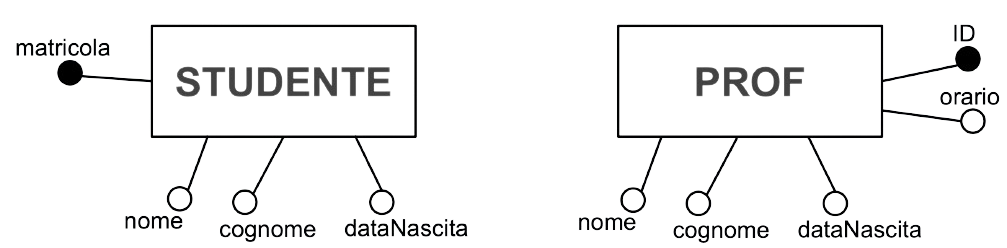
\includegraphics[width=.8\textwidth]{sections/er-model/img/generalization1.png}
    \end{center}
\end{frame}
%
\begin{frame}{Generalizzazione}
Le classi con attributi comuni possono essere generalizzate.
    \begin{center}
        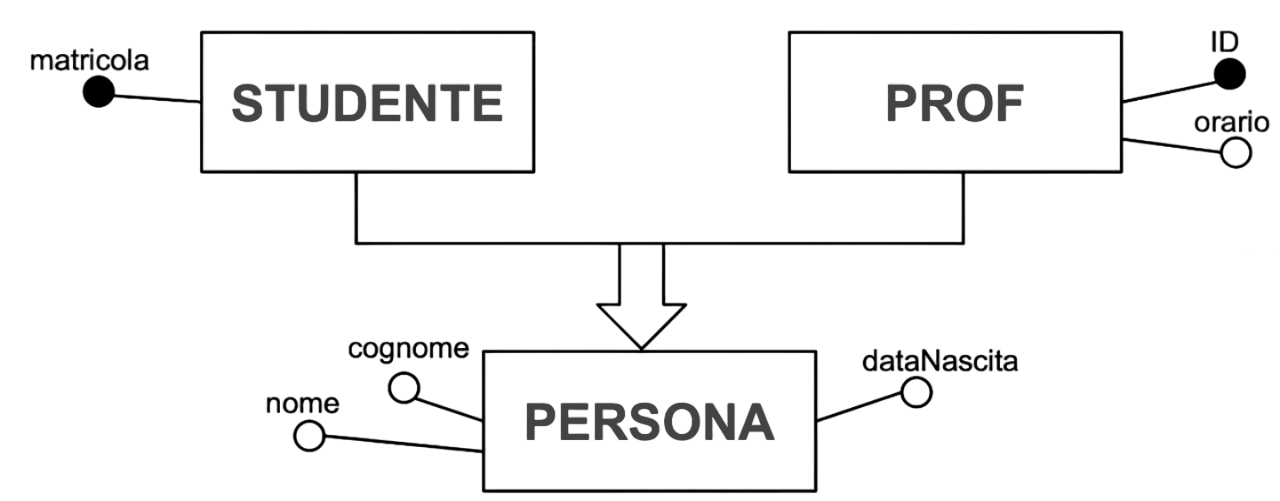
\includegraphics[width=.8\textwidth]{sections/er-model/img/generalization2.png}
    \end{center}
\end{frame}
%
\begin{frame}{Generalizzazione}
Altri simboli utilizzabili per i modelli E/R che a noi non interessano\ldots
    \begin{center}
        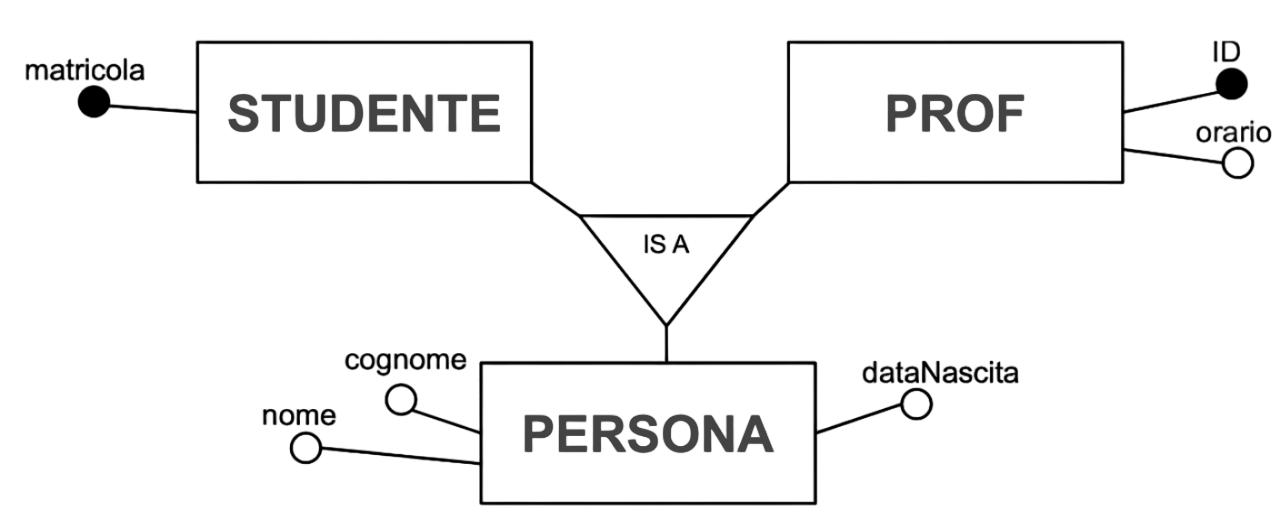
\includegraphics[width=.8\textwidth]{sections/er-model/img/generalization3.png}
    \end{center}
\end{frame}
%
\begin{frame}{Generalizzazione Parziale}
\begin{minipage}{.9\textwidth}
    \begin{block}{Generalizzazione Parziale}
        Una generalizzazione viene detta \textbf{parziale} se le specializzazioni non ricoprono tutti i casi possibili di una generalizzazione ma solamente alcuni.
    \end{block}
\end{minipage}
\begin{center}
    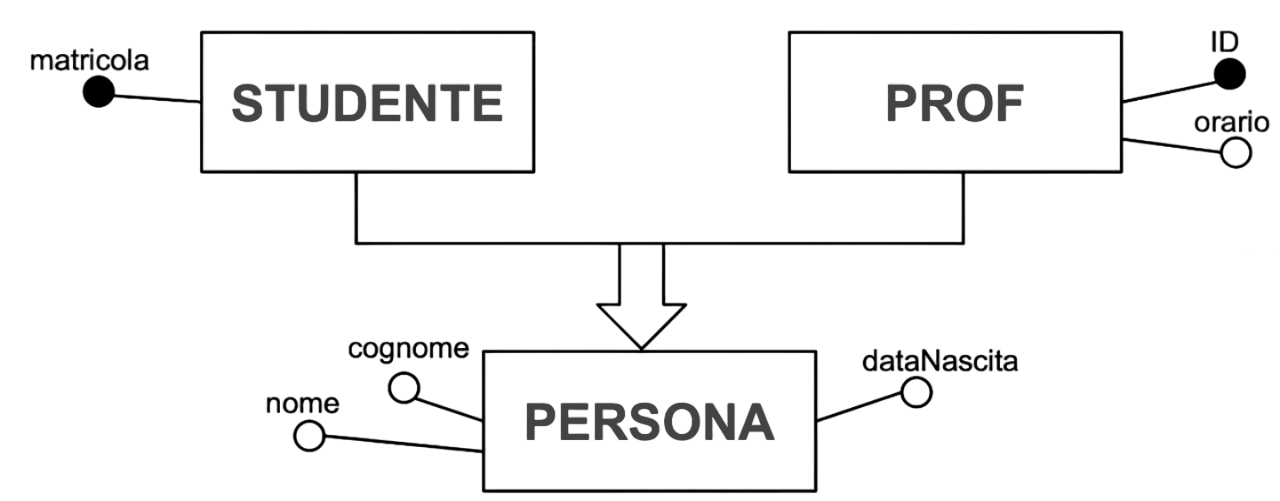
\includegraphics[width=.8\textwidth]{sections/er-model/img/generalization2.png}
\end{center}
\end{frame}
%
\begin{frame}{Generalizzazione Totale}
\begin{minipage}{.9\textwidth}
    \begin{block}{Generalizzazione Totale}
        Una generalizzazione viene detta \textbf{totale} se le specializzazioni ricoprono tutti i casi possibili di una generalizzazione.
    \end{block}
\end{minipage}
\begin{center}
    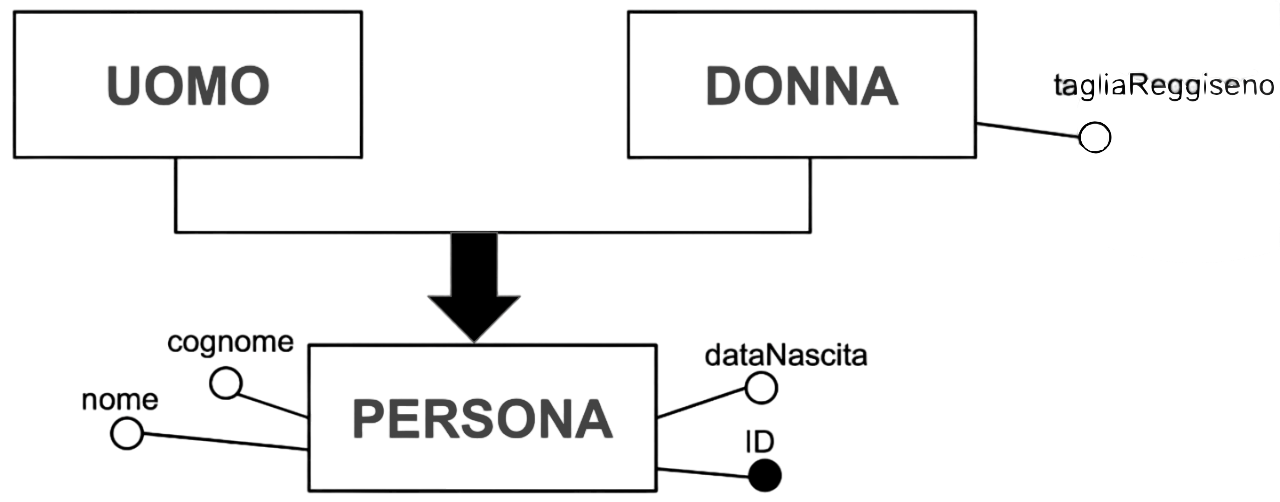
\includegraphics[width=.8\textwidth]{sections/er-model/img/generalization4.png}
\end{center}
\end{frame}
%
\begin{frame}{Generalizzazione Esclusiva}
\begin{minipage}{.9\textwidth}
    \begin{block}{Generalizzazione Esclusiva}
        Una generalizzazione viene detta \textbf{esclusiva} se le specializzazioni sono mutualmente esclusive.
    \end{block}
\end{minipage}
\begin{center}
    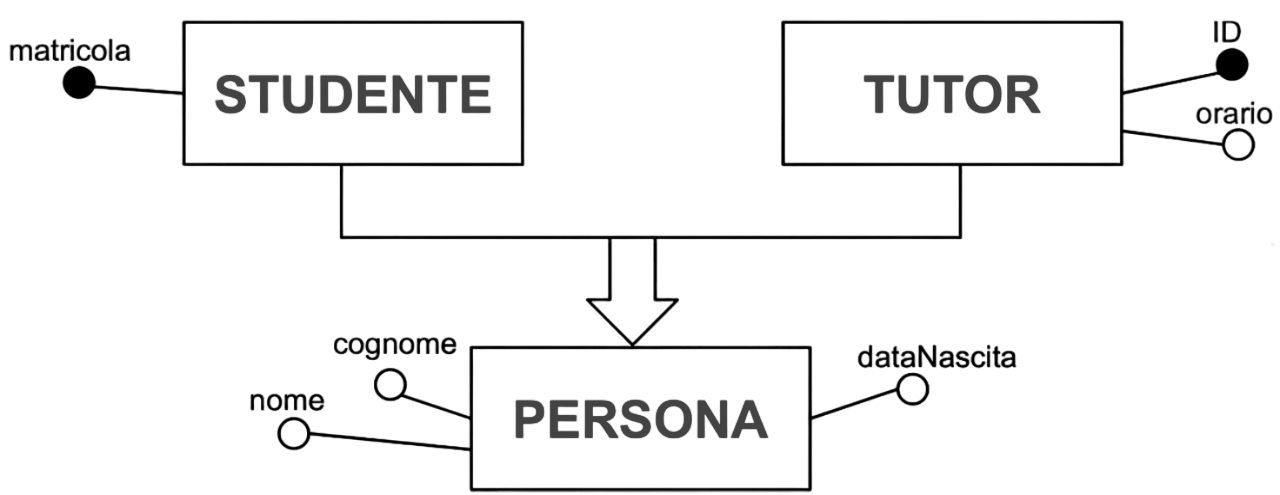
\includegraphics[width=.8\textwidth]{sections/er-model/img/generalization5.png}
\end{center}
\end{frame}
%
\begin{frame}{Generalizzazione}
Considerando tutte le combinazioni possibili delle propriet\`a appena viste possiamo avere 4 tipi di generalizzazione:
\begin{itemize}
    \item Totale Esclusiva (TE);
    \item Totale Sovrapposta (TS);
    \item Parziale Esclusiva (PE);
    \item Parziale Sovrapposta (PS).
\end{itemize}
\end{frame}